\renewcommand*{\arraystretch}{1.5}
\noindent\begin{tabularx}{17cm}{|p{1.95cm}|X|}
	\hline
	number      & 1                                                          \\ \hline
	title       & Posting summary                                                           \\ \hline
	\multicolumn{2}{|c|}{ 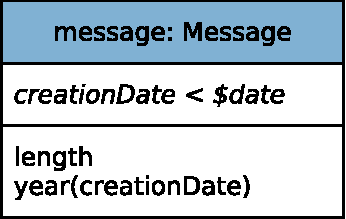
\includegraphics[scale=\patternscale,margin=0cm .2cm]{patterns/q01}} \\ \hline
	description & Given a date, find all Messages created before that date. Group them by
a 3-level grouping:

\begin{enumerate}
\def\labelenumi{\arabic{enumi}.}
\tightlist
\item
  by year of creation
\item
  for each year, group into message types, i.e., Posts or Comments
\item
  for each year-type group, split into four groups based on length of
  their content

  \begin{itemize}
  \tightlist
  \item
    0 \textless{}= length \textless{} 40: \texttt{short}
  \item
    40 \textless{}= length \textless{} 80: \texttt{one\ liner}
  \item
    80 \textless{}= length \textless{} 160: \texttt{tweet}
  \item
    160 \textless{}= length: \texttt{long}
  \end{itemize}
\end{enumerate}
 \\ \hline
	
	group by       &
	\multicolumn{1}{>{\raggedright}X|}{
		\varname{year}, 
		\varname{message type}, 
		\varname{length group}
		}\\ \hline
	
	parameters  &
	\renewcommand*{\arraystretch}{1.0}
	\vspace{-1.8ex}{\begin{tabularx}{14.2cm}{|c|l|p{2cm}|Y|} \hline
	\cellcolor{black!70} \color{white} $\mathsf{ 1 }$ & \varname{date} & \cellcolor{gray!20} \vartype{Date} & \\ 
	\end{tabularx}} \\ \hline
	result      &
	\renewcommand*{\arraystretch}{1.0}
	\vspace{-1.8ex}{\begin{tabularx}{14.2cm}{|c|l|p{2cm}|Y|} \hline
	\cellcolor{black!70} \color{white} $\mathsf{ 1 }$ & \varname{message.year} & \cellcolor{gray!20} \vartype{32bitInteger} & \\ \hline
	\cellcolor{black!70} \color{white} $\mathsf{ 2 }$ & \varname{messageType} & \cellcolor{gray!20} \vartype{String} &post/comment (in lowercase) \\ \hline
	\cellcolor{black!70} \color{white} $\mathsf{ 3 }$ & \varname{lengthCategory} & \cellcolor{gray!20} \vartype{String} &short/one-liner/tweet/long (in lowercase) \\ \hline
	\cellcolor{black!70} \color{white} $\mathsf{ 4 }$ & \varname{messageCount} & \cellcolor{gray!20} \vartype{32bitInteger} &total number of Messages (Posts/Comments) in that group \\ \hline
	\cellcolor{black!70} \color{white} $\mathsf{ 5 }$ & \varname{averageMessageLength} & \cellcolor{gray!20} \vartype{32bitInteger} &average length of the Message content in that group \\ \hline
	\cellcolor{black!70} \color{white} $\mathsf{ 6 }$ & \varname{sumMessageLength} & \cellcolor{gray!20} \vartype{32bitInteger} &sum of all message content lengths \\ \hline
	\cellcolor{black!70} \color{white} $\mathsf{ 7 }$ & \varname{percentageOfMessages} & \cellcolor{gray!20} \vartype{32bitFloat} &number of messages in group as a percentage of all messages created before the given date \\ 
	\end{tabularx}} \\ \hline
	sort        &
	\renewcommand*{\arraystretch}{1.0}
	\vspace{-1.8ex}{\begin{tabular}{|c|l|c|} \hline
	\cellcolor{black!70} \color{white} $\mathsf{ 1 }$ & \varname{year} & \cellcolor{gray!20} $\desc$ \\ \hline
	\cellcolor{black!70} \color{white} $\mathsf{ 2 }$ & \varname{message type} & \cellcolor{gray!20} $\asc$ \\ \hline
	\cellcolor{black!70} \color{white} $\mathsf{ 3 }$ & \varname{size category} & \cellcolor{gray!20} $\asc$ \\ 
	\end{tabular}} \\ \hline
	choke points        &
	\multicolumn{1}{>{\raggedright}X|}{
		\chokepoint{1.2}, 
		\chokepoint{3.2}, 
		\chokepoint{4.1}
		}\\ \hline
\end{tabularx}
\clearpage